
\documentclass[a3paper,12pt]{article} % Specify A3 paper size and font size
\usepackage{amsmath}
\usepackage{amssymb} % Include this package for \mathbb
\usepackage[margin=1in]{geometry} % Adjust the margin as needed
\usepackage{graphicx} % Include this package for \includegraphics

\begin{document}

\author{kipngeno koech - bkoech}
\title{Homework 6 - Mathetmatical Foundations of Machine Learning Engineers}
\maketitle

\medskip


\subsection*{1. Entropy of a Bernoulli Random Variable [10 points] } 

Consider a random variable $X$ that follows a Bernoulli distribution $B(1, p)$ with $0 < p < 1$. We define the entropy of $X$ as 
\[
H(p) = \mathbb{E}[-\log(p(X))].
\]
(You will need to read a little bit about entropy or consult a TA during office hours.)

\begin{enumerate}
    \item[(a)] Derive the second derivative $H''(p)$ of $H(p)$. If $H''(p) \leq 0$, $H(p)$ is called concave. Is $H(p)$ a concave function of $p$? \hfill (5 points)
    
    The probability mass function of a Bernoulli random variable is given by:
    \[
    p(x) = \begin{cases}
    p & \text{if } x = 1, \\
    1 - p & \text{if } x = 0.
    \end{cases}
    \]
    The expected value is given by:
    \[
    \mathbb{E}[X] = \sum_{x \in \{0, 1\}} x \cdot p(x).
    \]
    so the entropy of $X$ is:
    \[
    H(p) = -\sum_{x \in \{0, 1\}} p(x) \log(p(x)).
    \]
    this is equivalent to:
    \[
    H(p) = -p \log(p) - (1 - p) \log(1 - p).
    \]
    The first derivative of $H(p)$ with respect to $p$ is:
    \[
    H'(p) = -\log(p) - 1 + \log(1 - p).
    \]
    The second derivative of $H(p)$ with respect to $p$ is:
    \[
    H''(p) = -\frac{1}{p} - \frac{1}{1 - p}.
    \]
    The second derivative is always negative for $0 < p < 1$, so $H(p)$ is a concave function of $p$.
    \\ This means that the entropy of a Bernoulli random variable is a concave function of the probability $p$.
    \item[(b)] Find the value of $p \in (0, 1)$ that maximizes $H(p)$. \hfill (5 points)
    To maximize $H(p)$, we set the first derivative to zero:
    \[
    H'(p) = -\log(p) - 1 + \log(1 - p) = 0.
    \]
    \[
    \log(1 - p) - \log(p) = 1.
    \]
    \[
    \log\left(\frac{1 - p}{p}\right) = 1.
    \]
    \[
    {1 - p} = p
    \]
    \[
    p = \frac{1}{2}.
    \]
\end{enumerate}

\vspace{30pt}
\subsection*{2. Binary Classification with Logistic Regression [70 points]} 

Consider a binary classification problem where $y \in \{0, 1\}$ and $\mathbf{x} \in \mathbb{R}^2$. Our goal is to model $p(y = 1 \mid \mathbf{x})$. We decide to use a Bernoulli distribution parameterized by the random vector $\mathbf{w} \in \mathbb{R}^2$, such that:
\[
p_{\text{model}}(y = 1 \mid \mathbf{x}; \mathbf{w}) = \sigma(\mathbf{w}^\top \mathbf{x}),
\]
\[
p_{\text{model}}(y = 0 \mid \mathbf{x}; \mathbf{w}) = 1 - \sigma(\mathbf{w}^\top \mathbf{x}),
\]
where $\sigma(z) = \frac{1}{1 + e^{-z}}$ is the sigmoid function.

(a) Show that
\[
p_{\text{model}}(y \mid \mathbf{x}; \mathbf{w}) = \big(\sigma(\mathbf{w}^\top \mathbf{x})\big)^y \big(1 - \sigma(\mathbf{w}^\top \mathbf{x})\big)^{1-y}.
\]
\hfill (5 points)

The probability mass function of a Bernoulli random variable is given by:
\[
p(y \mid \mathbf{x}; \mathbf{w}) = \begin{cases}
\sigma(\mathbf{w}^\top \mathbf{x}) & \text{if } y = 1, \\
1 - \sigma(\mathbf{w}^\top \mathbf{x}) & \text{if } y = 0.
\end{cases}
\]
This is equivalent to:

\[
p(y \mid \mathbf{x}; \mathbf{w}) = \big(\sigma(\mathbf{w}^\top \mathbf{x})\big)^y \big(1 - \sigma(\mathbf{w}^\top \mathbf{x})\big)^{1-y}.
\]
This is because:
\[
\sigma(\mathbf{w}^\top \mathbf{x})^1 = \sigma(\mathbf{w}^\top \mathbf{x}), \quad \sigma(\mathbf{w}^\top \mathbf{x})^0 = 1 - \sigma(\mathbf{w}^\top \mathbf{x}).
\]

(b)
Table 1 contains 10 samples, $(\mathbf{x}, y)$, obtained from the data-generating distribution $p_{\text{data}}$. The KL divergence between $p_{\text{data}}$ and $p_{\text{model}}$ is given as:
\[
D_{\text{KL}}(p_{\text{data}} \mid\mid p_{\text{model}}) = \mathbb{E}_{\mathbf{x}, y \sim p_{\text{data}}} \big[\log p_{\text{data}}(y \mid \mathbf{x}) - \log p_{\text{model}}(y \mid \mathbf{x})\big].
\]

The cross entropy of $p_{\text{data}}$ and $p_{\text{model}}$ is:
\[
-\mathbb{E}_{\mathbf{x}, y \sim p_{\text{data}}} \big[\log p_{\text{model}}(y \mid \mathbf{x})\big].
\]

Given empirical data as in Table 1, show that the cross entropy satisfies the expression:
\[
-\mathbb{E}_{\mathbf{x}, y \sim p_{\text{data}}} \big[\log p_{\text{model}}(y \mid \mathbf{x})\big] = -\frac{1}{N} \sum^N_{i=1} \big[y_i \log(\sigma(\mathbf{w}^\top \mathbf{x_i})) + (1-y_i) \log(1-\sigma(\mathbf{w}^\top \mathbf{x_i}))\big].
\]
\hfill (5 points)

\begin{table}[h!]
\centering
\begin{tabular}{|c|c|c|}
\hline
\textbf{Sample} & $\mathbf{x}$ & $\mathbf{y}$ \\ \hline
1 & $[-1, 4]$ & 1 \\ \hline
2 & $[-3, 2]$ & 0 \\ \hline
3 & $[-2, 1]$ & 0 \\ \hline
4 & $[1, 2]$ & 1 \\ \hline
5 & $[2, 1]$ & 1 \\ \hline
6 & $[-1, 1]$ & 0 \\ \hline
7 & $[-2, -2]$ & 0 \\ \hline
8 & $[1, -2]$ & 0 \\ \hline
9 & $[3, -1]$ & 1 \\ \hline
10 & $[2, 0]$ & 1 \\ \hline
\end{tabular}
\caption{Samples $(\mathbf{x}, y)$ obtained from the data-generating distribution $p_{\text{data}}$.}
\label{tab:table1}
\end{table}
\(\textbf{solution:}\)
The cross entropy of $p_{\text{data}}$ and $p_{\text{model}}$ is given by:
\[
-\mathbb{E}_{\mathbf{x}, y \sim p_{\text{data}}} \big[\log p_{\text{model}}(y \mid \mathbf{x})\big].
\]
for binary classification, y can either be zero or one. The cross entropy is given by:
\[
-\mathbb{E}_{\mathbf{x}, y \sim p_{\text{data}}} \big[\log p_{\text{model}}(y \mid \mathbf{x})\big] = -\mathbb{E}_{\mathbf{x}, y \sim p_{\text{data}}} \big[y \log(\sigma(\mathbf{w}^\top \mathbf{x})) + (1-y) \log(1-\sigma(\mathbf{w}^\top \mathbf{x}))\big].
\]
The cross entropy is the negative log-likelihood of the data given the model. The likelihood of the data given the model is:
\[
p_{\text{model}}(y \mid \mathbf{x}) = \big(\sigma(\mathbf{w}^\top \mathbf{x})\big)^y \big(1 - \sigma(\mathbf{w}^\top \mathbf{x})\big)^{1-y}.
\]
The cross entropy is the negative log-likelihood of the data given the model:
\[
-\mathbb{E}_{\mathbf{x}, y \sim p_{\text{data}}} \big[\log p_{\text{model}}(y \mid \mathbf{x})\big] = -\frac{1}{N} \sum^N_{i=1} \big[y_i \log(\sigma(\mathbf{w}^\top \mathbf{x_i})) + (1-y_i) \log(1-\sigma(\mathbf{w}^\top \mathbf{x_i}))\big].
\]

(c)
Minimizing the cross entropy of $p_{\text{data}}$ and $p_{\text{model}}$ implies that $p_{\text{model}}$ will approximate the data-generating distribution. We define the loss function of our model as:
\[
L(\mathbf{w}) = -\frac{1}{N} \sum^N_{i=1} \big[y_i \log(\sigma(\mathbf{w}^\top \mathbf{x_i})) + (1-y_i) \log(1-\sigma(\mathbf{w}^\top \mathbf{x_i}))\big].
\]
Obtain an expression for the gradient of $L(\mathbf{w})$ with respect to $\mathbf{w}$, and show that $L(\mathbf{w})$ is a convex function.
\hfill (10 points)

the loss function is given by:
\[
L(\mathbf{w}) = -\frac{1}{N} \sum^N_{i=1} \big[y_i \log(\sigma(\mathbf{w}^\top \mathbf{x_i})) + (1-y_i) \log(1-\sigma(\mathbf{w}^\top \mathbf{x_i}))\big].
\]
The gradient of the loss function with respect to $\mathbf{w}$ is:
\[
\nabla L(\mathbf{w}) = -\frac{1}{N} \sum^N_{i=1} \big[y_i \frac{\sigma(\mathbf{w}^\top \mathbf{x_i})(1 - \sigma(\mathbf{w}^\top \mathbf{x_i}))}{\sigma(\mathbf{w}^\top \mathbf{x_i})} \mathbf{x_i} - (1-y_i) \frac{\sigma(\mathbf{w}^\top \mathbf{x_i})(1 - \sigma(\mathbf{w}^\top \mathbf{x_i}))}{1 - \sigma(\mathbf{w}^\top \mathbf{x_i})} \mathbf{x_i}\big].
\]
\[
\nabla L(\mathbf{w}) = -\frac{1}{N} \sum^N_{i=1} \big[y_i (1 - \sigma(\mathbf{w}^\top \mathbf{x_i})) \mathbf{x_i} - (1-y_i) \sigma(\mathbf{w}^\top \mathbf{x_i}) \mathbf{x_i}\big].
\]
\[
\nabla L(\mathbf{w}) = -\frac{1}{N} \sum^N_{i=1} \big[y_i - \sigma(\mathbf{w}^\top \mathbf{x_i})\big] \mathbf{x_i}.
\]
To show that $L(\mathbf{w})$ is a convex function, we need to show that the Hessian matrix is positive semi-definite. The Hessian matrix is given by:
\[
\nabla^2 L(\mathbf{w}) = \frac{1}{N} \sum^N_{i=1} \sigma(\mathbf{w}^\top \mathbf{x_i}) \big(1 - \sigma(\mathbf{w}^\top \mathbf{x_i})\big) \mathbf{x_i} \mathbf{x_i}^\top.
\]

The Hessian matrix is positive semi-definite if:
\[
\mathbf{v}^\top \nabla^2 L(\mathbf{w}) \mathbf{v} \geq 0, \quad \forall \mathbf{v} \in \mathbb{R}^2.
\]
\[
\mathbf{v}^\top \nabla^2 L(\mathbf{w}) \mathbf{v} = \frac{1}{N} \sum^N_{i=1} \sigma(\mathbf{w}^\top \mathbf{x_i}) \big(1 - \sigma(\mathbf{w}^\top \mathbf{x_i})\big) \mathbf{v}^\top \mathbf{x_i} \mathbf{x_i}^\top \mathbf{v} \geq 0.
\]
The Hessian matrix is positive semi-definite, so $L(\mathbf{w})$ is a convex function.

(d)
The gradient expression obtained above can be seen as the empirical mean of the gradient for each sample $i$. \(\nabla L(w) = \frac{1}{N}\sum^N_{i=1}\nabla L_i(w)\). Given that the gradient for each sample is independent and identically distributed with variance $\sigma_g^2$, Show that the standard error of the gradient given $n$ samples from the data-generating distribution is \[SE = \frac{\sigma_g}{\sqrt{n}}\] 
Explain why a better estimate of the gradient is obtained by increasing the number of samples.

\hfill (5 points)

The standard error of the gradient is given by:
\[
SE = \frac{\sigma_g}{\sqrt{n}}.
\]
The variance of the gradient is given by:
\[
\text{Var}(\nabla L_i(\mathbf{w})) = \sigma_g^2.
\]
The variance of the gradient for $n$ samples is:
\[
\text{Var}(\nabla L(\mathbf{w})) = \frac{1}{N} \sum^N_{i=1} \text{Var}(\nabla L_i(\mathbf{w})) = \frac{1}{N} \sum^N_{i=1} \sigma_g^2 = \sigma_g^2.
\]
The standard error of the gradient is:
\[
SE = \sqrt{\text{Var}(\nabla L(\mathbf{w}))} = \sqrt{\sigma_g^2} = \sigma_g.
\]
The standard error of the gradient is inversely proportional to the square root of the number of samples. A better estimate of the gradient is obtained by increasing the number of samples because the standard error of the gradient decreases as the number of samples increases. This means that the gradient estimate becomes more accurate with more samples.

\(\newline\)
(e)
Stochastic gradient descent (SGD) with a minibatch computes the gradient using only a subset of the total samples when performing parameter updates. The minibatch size, $m$, is always less than the total number of samples, $N$. Given that an epoch of updates involves using all available samples:
\begin{itemize}
    \item Perform SGD updates for 1 epoch while reporting the values of the loss and the parameters after each update in the format shown in Table 2.
    \item Use a learning rate of 0.1 and a minibatch size of 2.
    \item start with \(\mathbf{w} = [0,0]\)
\end{itemize}
The SGD update is given as:
\[ w \gets w - \alpha\nabla L(\mathbf{w})\]
\textbf{Note: You must show all your workings to get full points.}
\hfill (20 points)

\(\textbf{solution:}\)
minibatch size, \(m = 2\)
learning rate, \(\alpha = 0.1\)
initial parameters, \(\mathbf{w} = [0, 0]\)
activation function, \(\sigma(z) = \frac{1}{1 + e^{-z}}\)

\textbf{Minibatch 1:}
items in minibatch 1: \(\{1, 2\}\), \(\mathbf{x_1} = [-1, 4]\), \(y_1 = 1\), \(\mathbf{x_2} = [-3, 2]\), \(y_2 = 0\)
\\ Forward pass:
\[
\sigma(\mathbf{w}^\top \mathbf{x_1}) = \sigma([0, 0] \cdot [-1, 4]) = \sigma(0) = \sigma(z) = \frac{1}{1 + e^{-z}} = \frac{1}{1 + e^{0}} = \frac{1}{2} = 0.5
\]
\[
\sigma(\mathbf{w}^\top \mathbf{x_2}) = \sigma([0, 0] \cdot [-3, 2]) = \sigma(0) = \sigma(z) = \frac{1}{1 + e^{-z}} = \frac{1}{1 + e^{0}} = \frac{1}{2} = 0.5
\]
The p model is:
\[
p_{\text{model}}(y \mid \mathbf{x}; \mathbf{w}) = \big(\sigma(\mathbf{w}^\top \mathbf{x})\big)^y \big(1 - \sigma(\mathbf{w}^\top \mathbf{x})\big)^{1-y}.
\]
so:
\[
p_{\text{model}}(y_1 \mid \mathbf{x_1}; \mathbf{w}) = \big(\sigma(\mathbf{w}^\top \mathbf{x_1})\big)^{y_1} \big(1 - \sigma(\mathbf{w}^\top \mathbf{x_1})\big)^{1-y_1} = (0.5)^1 (0.5)^0 = 0.5
\]
\[
p_{\text{model}}(y_2 \mid \mathbf{x_2}; \mathbf{w}) = \big(\sigma(\mathbf{w}^\top \mathbf{x_2})\big)^{y_2} \big(1 - \sigma(\mathbf{w}^\top \mathbf{x_2})\big)^{1-y_2} = (0.5)^0 (0.5)^1 = 0.5
\]
The loss gradient function is:
\[
\nabla L(\mathbf{w}) = -\frac{1}{N} \sum^N_{i=1} \big[y_i - \sigma(\mathbf{w}^\top \mathbf{x_i})\big] \mathbf{x_i}.
\]
so the backward pass is:
\[
\nabla L(\mathbf{w}) = -\frac{1}{2} \sum^2_{i=1} \big[y_i - \sigma(\mathbf{w}^\top \mathbf{x_i})\big] \mathbf{x_i}.
\]
\[
\nabla L(\mathbf{w}) = -\frac{1}{2} \big[y_1 - \sigma(\mathbf{w}^\top \mathbf{x_1})\big] \mathbf{x_1} - \frac{1}{2} \big[y_2 - \sigma(\mathbf{w}^\top \mathbf{x_2})\big] \mathbf{x_2}.
\]
\[
\nabla L(\mathbf{w}) = -\frac{1}{2} \big[1 - 0.5\big] [-1, 4] - \frac{1}{2} \big[0 - 0.5\big] [-3, 2].
\]
\[
\nabla L(\mathbf{w}) = -\frac{1}{2} \big[0.5\big] [-1, 4] - \frac{1}{2} \big[-0.5\big] [-3, 2].
\]
\[
\nabla L(\mathbf{w}) = -\frac{1}{2} [-0.5, 2] + \frac{1}{2} [1.5, -1].
\]
\[
\nabla L(\mathbf{w}) = [0.25, -1] + [-0.75, 0.5]. = [-0.5, -0.5].
\]  
The updated parameters are:
\[
\mathbf{w} \gets \mathbf{w} - \alpha \nabla L(\mathbf{w}) = [0, 0] - 0.1 [-0.5, -0.5] = [0, 0] - [-0.05, -0.05] = [0.05, 0.05].
\]
The loss is:
\[
L(\mathbf{w}) = -\frac{1}{2} \sum^2_{i=1} \big[y_i \log(\sigma(\mathbf{w}^\top \mathbf{x_i})) + (1-y_i) \log(1-\sigma(\mathbf{w}^\top \mathbf{x_i}))\big].
\]
The loss then is:
\[
L(\mathbf{w}) = -\frac{1}{2} \big[1 \ln(0.5) + (1-1) \ln(1-0.5)\big] - \frac{1}{2} \big[0 \ln(0.5) + (1-0) \ln(1-0.5)\big].
\]
\[
L(\mathbf{w}) = -\frac{1}{2} \big[1 \ln(0.5) + 0 \ln(0.5)\big] - \frac{1}{2} \big[0 \ln(0.5) + 1 \ln(0.5)\big].
\]
\[
L(\mathbf{w}) = -\frac{1}{2} \big[-0.693147 + 0\big] - \frac{1}{2} \big[0 + -0.693147\big].
\]
\[
L(\mathbf{w}) = -\frac{1}{2} \big[-0.693147\big] - \frac{1}{2} \big[-0.693147\big].
\]
\[
L(\mathbf{w}) = 0.693147.
\]
The updated parameters are \(\mathbf{w} = \mathbf{[0.05, 0.05]}\) and the loss is \(L(\mathbf{w}) = \mathbf{0.693147}\).
\\ \textbf{Minibatch 2:}
\\ items in minibatch 2: \(\{3, 4\}\), \(\mathbf{x_3} = [-2, 1]\), \(y_3 = 0\), \(\mathbf{x_4} = [1, 2]\), \(y_4 = 1\)
\\ Forward pass:
\[
\sigma(\mathbf{w}^\top \mathbf{x_3}) = \sigma([0.05, 0.05] \cdot [-2, 1]) = \sigma(-0.1 + 0.05) = \sigma(-0.05) = 0.4875
\]
\[
\sigma(\mathbf{w}^\top \mathbf{x_4}) = \sigma([0.05, 0.05] \cdot [1, 2]) = \sigma(0.05 + 0.1) = \sigma(0.15) = 0.5375
\]
The p model is:
\[
p_{\text{model}}(y_3 \mid \mathbf{x_3}; \mathbf{w}) = \big(\sigma(\mathbf{w}^\top \mathbf{x_3})\big)^{y_3} \big(1 - \sigma(\mathbf{w}^\top \mathbf{x_3})\big)^{1-y_3} = (0.4875)^0 (0.5125)^1 = 0.5125
\]
\[
p_{\text{model}}(y_4 \mid \mathbf{x_4}; \mathbf{w}) = \big(\sigma(\mathbf{w}^\top \mathbf{x_4})\big)^{y_4} \big(1 - \sigma(\mathbf{w}^\top \mathbf{x_4})\big)^{1-y_4} = (0.5375)^1 (0.4625)^0 = 0.5375
\]
The loss gradient function is:
\[
\nabla L(\mathbf{w}) = -\frac{1}{N} \sum^N_{i=1} \big[y_i - \sigma(\mathbf{w}^\top \mathbf{x_i})\big] \mathbf{x_i}.
\]
so the backward pass is:
\[
\nabla L(\mathbf{w}) = -\frac{1}{2} \sum^2_{i=1} \big[y_i - \sigma(\mathbf{w}^\top \mathbf{x_i})\big] \mathbf{x_i}.
\]
\[
\nabla L(\mathbf{w}) = -\frac{1}{2} \big[y_3 - \sigma(\mathbf{w}^\top \mathbf{x_3})\big] \mathbf{x_3} - \frac{1}{2} \big[y_4 - \sigma(\mathbf{w}^\top \mathbf{x_4})\big] \mathbf{x_4}.
\]
\[
\nabla L(\mathbf{w}) = -\frac{1}{2} \big[0 - 0.4875\big] [-2, 1] - \frac{1}{2} \big[1 - 0.5375\big] [1, 2].
\]
\[
\nabla L(\mathbf{w}) = -\frac{1}{2} \big[-0.4875\big] [-2, 1] - \frac{1}{2} \big[0.4625\big] [1, 2].
\]
\[
\nabla L(\mathbf{w}) = -\frac{1}{2} [0.975, -0.4875] - \frac{1}{2} [0.4625, 0.925].
\]
\[
\nabla L(\mathbf{w}) = [-0.4875, 0.2438] - [0.2313, 0.4625]. = [-0.7188, -0.2188].
\]
The updated parameters are:
\[
\mathbf{w} \gets \mathbf{w} - \alpha \nabla L(\mathbf{w}) = [0.05, 0.05] - 0.1 [-0.7188, -0.2188] = [0.05, 0.05] - [-0.0719, -0.0219] = [0.1219, 0.0719].
\]
The loss is:
\[
L(\mathbf{w}) = -\frac{1}{2} \sum^2_{i=1} \big[y_i \log(\sigma(\mathbf{w}^\top \mathbf{x_i})) + (1-y_i) \log(1-\sigma(\mathbf{w}^\top \mathbf{x_i}))\big].
\]

The loss then is:
\[
L(\mathbf{w}) = -\frac{1}{2} \big[0 \ln(0.4875) + (1-0) \ln(1-0.4875)\big] - \frac{1}{2} \big[1 \ln(0.5375) + (1-1) \ln(1-0.5375)\big].
\]
\[
L(\mathbf{w}) = -\frac{1}{2} \big[0 \ln(0.4875) + 1 \ln(0.5125)\big] - \frac{1}{2} \big[1 \ln(0.5375) + 0 \ln(0.4625)\big].
\]
\[
L(\mathbf{w}) = -\frac{1}{2} \big[0 + -0.66845\big] - \frac{1}{2} \big[-0.6208 + 0\big].
\]
\[
L(\mathbf{w}) = -\frac{1}{2} \big[-0.6845\big] - \frac{1}{2} \big[-0.6208\big].
\]
\[
L(\mathbf{w}) = 0.65265.
\]
The updated parameters are \(\mathbf{w} = \mathbf{[0.1219, 0.0719]}\) and the loss is \(L(\mathbf{w}) = \mathbf{0.6255}\).
\\ \textbf{Minibatch 3:}
\\ items in minibatch 3: \(\{5, 6\}\), \(\mathbf{x_5} = [2, 1]\), \(y_5 = 1\), \(\mathbf{x_6} = [-1, 1]\), \(y_6 = 0\)
\\ Forward pass:
\[
\sigma(\mathbf{w}^\top \mathbf{x_5}) = \sigma([0.1219, 0.0719] \cdot [2, 1]) = \sigma(0.2438 + 0.0719) = \sigma(0.3157) = 0.5783
\]
\[
\sigma(\mathbf{w}^\top \mathbf{x_6}) = \sigma([0.1219, 0.0719] \cdot [-1, 1]) = \sigma(-0.1219 + 0.0719) = \sigma(-0.05) = 0.4875
\]
The p model is:
\[
p_{\text{model}}(y_5 \mid \mathbf{x_5}; \mathbf{w}) = \big(\sigma(\mathbf{w}^\top \mathbf{x_5})\big)^{y_5} \big(1 - \sigma(\mathbf{w}^\top \mathbf{x_5})\big)^{1-y_5} = (0.5783)^1 (0.4217)^0 = 0.5783
\]
\[
p_{\text{model}}(y_6 \mid \mathbf{x_6}; \mathbf{w}) = \big(\sigma(\mathbf{w}^\top \mathbf{x_6})\big)^{y_6} \big(1 - \sigma(\mathbf{w}^\top \mathbf{x_6})\big)^{1-y_6} = (0.4875)^0 (0.5125)^1 = 0.5125
\]
The loss gradient function is:
\[
\nabla L(\mathbf{w}) = -\frac{1}{N} \sum^N_{i=1} \big[y_i - \sigma(\mathbf{w}^\top \mathbf{x_i})\big] \mathbf{x_i}.
\]
so the backward pass is:
\[
\nabla L(\mathbf{w}) = -\frac{1}{2} \sum^2_{i=1} \big[y_i - \sigma(\mathbf{w}^\top \mathbf{x_i})\big] \mathbf{x_i}.
\]
\[
\nabla L(\mathbf{w}) = -\frac{1}{2} \big[y_5 - \sigma(\mathbf{w}^\top \mathbf{x_5})\big] \mathbf{x_5} - \frac{1}{2} \big[y_6 - \sigma(\mathbf{w}^\top \mathbf{x_6})\big] \mathbf{x_6}.
\]
\[
\nabla L(\mathbf{w}) = -\frac{1}{2} \big[[1 - 0.5783] [2, 1] -  \big[0 - 0.5125\big] [-1, 1]\big]
\]
\[
\nabla L(\mathbf{w}) = -\frac{1}{2} \big[0.4217] [2, 1] - \frac{1}{2} \big[-0.5125] [-1, 1].
\]
\[
\nabla L(\mathbf{w}) = [-0.4217, -0.2108] - [0.25625, -0.25625]. = [-0.67795, 0.04545].
\]
The updated parameters are:
\[
\mathbf{w} \gets \mathbf{w} - \alpha \nabla L(\mathbf{w}) = [0.1219, 0.0719] - 0.1 [-0.67795, -0.4545] = [0.1219, 0.0719] - [-0.067795, -0.04545] = [0.1885, 0.064].
\]
The loss is:
\[
L(\mathbf{w}) = -\frac{1}{2} \sum^2_{i=1} \big[y_i \ln(\sigma(\mathbf{w}^\top \mathbf{x_i})) + (1-y_i) \ln(1-\sigma(\mathbf{w}^\top \mathbf{x_i}))\big].
\]

The loss then is:
\[
L(\mathbf{w}) = -\frac{1}{2} \big[1 \ln(0.5783) + (1-1) \ln(1-0.5783)\big] - \frac{1}{2} \big[0 \ln(0.4875) + (1-0) \ln(1-0.4822)\big].
\]
\[
L(\mathbf{w}) = -\frac{1}{2} \big[1 \ln(0.5783) + 0 \ln(0.4217)\big] - \frac{1}{2} \big[0 \ln(0.4822) + 1 \ln(0.5125)\big].
\]
\[
L(\mathbf{w}) = -\frac{1}{2} \big[-0.54766 + 0\big] - \frac{1}{2} \big[0 + -0.66845\big].
\]
\[
L(\mathbf{w}) = -\frac{1}{2} \big[-0.54766\big] - \frac{1}{2} \big[-0.2858\big].
\]
\[
L(\mathbf{w}) = 0.608055.
\]
The updated parameters are \(\mathbf{w} = \mathbf{[0.1885, 0.064]}\) and the loss is \(L(\mathbf{w}) = \mathbf{0.608055}\).
\\ \textbf{Minibatch 4:}
\\ items in minibatch 4: \(\{7, 8\}\), \(\mathbf{x_7} = [-2, -2]\), \(y_7 = 0\), \(\mathbf{x_8} = [1, -2]\), \(y_8 = 0\)
\\ Forward pass:
\[
\sigma(\mathbf{w}^\top \mathbf{x_7}) = \sigma([0.1885, 0.064] \cdot [-2, -2]) = \sigma(-0.377 + -0.128) = \sigma(-0.505) = 0.376366
\]
\[
\sigma(\mathbf{w}^\top \mathbf{x_8}) = \sigma([0.1885, 0.064] \cdot [1, -2]) = \sigma(0.1885 - 0.2348) = \sigma(0.0605) = 0.51512
\]
The p model is:
\[
p_{\text{model}}(y_7 \mid \mathbf{x_7}; \mathbf{w}) = \big(\sigma(\mathbf{w}^\top \mathbf{x_7})\big)^{y_7} \big(1 - \sigma(\mathbf{w}^\top \mathbf{x_7})\big)^{1-y_7} = (0.376366)^0 (0.623634)^1 = 0.623634
\]
\[
p_{\text{model}}(y_8 \mid \mathbf{x_8}; \mathbf{w}) = \big(\sigma(\mathbf{w}^\top \mathbf{x_8})\big)^{y_8} \big(1 - \sigma(\mathbf{w}^\top \mathbf{x_8})\big)^{1-y_8} = (0.51512)^0 (0.4848796)^1 = 0.4848796
\]
The loss gradient function is:
\[
\nabla L(\mathbf{w}) = -\frac{1}{N} \sum^N_{i=1} \big[y_i - \sigma(\mathbf{w}^\top \mathbf{x_i})\big] \mathbf{x_i}.
\]
so the backward pass is:
\[
\nabla L(\mathbf{w}) = -\frac{1}{2} \sum^2_{i=1} \big[y_i - \sigma(\mathbf{w}^\top \mathbf{x_i})\big] \mathbf{x_i}.
\]
\[
\nabla L(\mathbf{w}) = -\frac{1}{2} \big[y_7 - \sigma(\mathbf{w}^\top \mathbf{x_7})\big] \mathbf{x_7} - \frac{1}{2} \big[y_8 - \sigma(\mathbf{w}^\top \mathbf{x_8})\big] \mathbf{x_8}.
\]
\[
\nabla L(\mathbf{w}) = -\frac{1}{2} \big[0 - 0.376366\big] [-2, -2] - \frac{1}{2} \big[0 - 0.51512\big] [1, -2].
\]
\[
\nabla L(\mathbf{w}) = -\frac{1}{2} \big[-0.376366] [-2, -2] - \frac{1}{2} \big[-0.51512] [1, -2].
\]
\[
\nabla L(\mathbf{w}) = [0.376366, 0.376366] - [-0.25756, 0.51512]. = [0.633926, -0.138754].
\]
The updated parameters are:
\[
\mathbf{w} \gets \mathbf{w} - \alpha \nabla L(\mathbf{w}) = [0.1885, 0.1174] - 0.1 [0.633926, -0.138754] = [0.1885, -0.0138754] - [0.063339, 0.0215] = [0.20, 0.1514].
\]
The loss is:
\[
L(\mathbf{w}) = -\frac{1}{2} \sum^2_{i=1} \big[y_i \log(\sigma(\mathbf{w}^\top \mathbf{x_i})) + (1-y_i) \log(1-\sigma(\mathbf{w}^\top \mathbf{x_i}))\big].
\]
for the seventh data point:
\[
    \sigma(\mathbf{w}^\top \mathbf{x_i}) = \sigma([0.0937, 0.0959] \cdot [-2, -2]) = \sigma(-0.1874 - 0.1918) = \sigma(-0.3792) = 0.4063
\]
for the eighth data point:
\[
    \sigma(\mathbf{w}^\top \mathbf{x_i}) = \sigma([0.0937, 0.0959] \cdot [1, -2]) = \sigma(0.0937 - 0.1918) = \sigma(-0.0981) = 0.4755
\]
The loss then is:
\[
L(\mathbf{w}) = -\frac{1}{2} \big[0 \log(0.4063) + (1-0) \log(1-0.4063)\big] - \frac{1}{2} \big[0 \log(0.4755) + (1-0) \log(1-0.4755)\big].
\]
\[
L(\mathbf{w}) = -\frac{1}{2} \big[0 \log(0.4063) + 1 \log(0.5937)\big] - \frac{1}{2} \big[0 \log(0.4755) + 1 \log(0.5245)\big].
\]
\[
L(\mathbf{w}) = -\frac{1}{2} \big[0 + -0.2264\big] - \frac{1}{2} \big[0 + -0.28025\big].
\]
\[
L(\mathbf{w}) = -\frac{1}{2} \big[-0.2264\big] - \frac{1}{2} \big[-0.28025\big].
\]
\[
L(\mathbf{w}) = 0.2533.
\]
The updated parameters are \(\mathbf{w} = \mathbf{[0.0937, 0.0959]}\) and the loss is \(L(\mathbf{w}) = \mathbf{0.2533}\).
\\ \textbf{Minibatch 5:}
\\ items in minibatch 5: \(\{9, 10\}\), \(\mathbf{x_9} = [1, -1]\), \(y_9 = 1\), \(\mathbf{x_{10}} = [2, -2]\), \(y_{10} = 0\)
\\ Forward pass:
\[
\sigma(\mathbf{w}^\top \mathbf{x_9}) = \sigma([0.0937, 0.0959] \cdot [1, -1]) = \sigma(0.0937 - 0.0959) = \sigma(-0.0022) = 0.4995
\]
\[
\sigma(\mathbf{w}^\top \mathbf{x_{10}}) = \sigma([0.0937, 0.0959] \cdot [2, -2]) = \sigma(0.1874 - 0.1918) = \sigma(-0.0044) = 0.4989
\]
The p model is:
\[
p_{\text{model}}(y_9 \mid \mathbf{x_9}; \mathbf{w}) = \big(\sigma(\mathbf{w}^\top \mathbf{x_9})\big)^{y_9} \big(1 - \sigma(\mathbf{w}^\top \mathbf{x_9})\big)^{1-y_9} = (0.4995)^1 (0.5005)^0 = 0.4995
\]
\[
p_{\text{model}}(y_{10} \mid \mathbf{x_{10}}; \mathbf{w}) = \big(\sigma(\mathbf{w}^\top \mathbf{x_{10}})\big)^{y_{10}} \big(1 - \sigma(\mathbf{w}^\top \mathbf{x_{10}})\big)^{1-y_{10}} = (0.4989)^0 (0.5011)^1 = 0.5011
\]
The loss gradient function is:
\[
\nabla L(\mathbf{w}) = -\frac{1}{N} \sum^N_{i=1} \big[y_i - \sigma(\mathbf{w}^\top \mathbf{x_i})\big] \mathbf{x_i}.
\]
so the backward pass is:
\[
\nabla L(\mathbf{w}) = -\frac{1}{2} \sum^2_{i=1} \big[y_i - \sigma(\mathbf{w}^\top \mathbf{x_i})\big] \mathbf{x_i}.
\]
\[
\nabla L(\mathbf{w}) = -\frac{1}{2} \big[y_9 - \sigma(\mathbf{w}^\top \mathbf{x_9})\big] \mathbf{x_9} - \frac{1}{2} \big[y_{10} - \sigma(\mathbf{w}^\top \mathbf{x_{10}})\big] \mathbf{x_{10}}.
\]
\[
\nabla L(\mathbf{w}) = -\frac{1}{2} \big[1 - 0.4995\big] [1, -1] - \frac{1}{2} \big[0 - 0.5011\big] [2, -2].
\]
\[
\nabla L(\mathbf{w}) = -\frac{1}{2} \big[0.5005] [1, -1] - \frac{1}{2} \big[-0.5011] [2, -2].
\]
\[
\nabla L(\mathbf{w}) = -\frac{1}{2}[0.5005, -0.5005] -\frac{1}{2} [-1.0022, 1.0022]. = [-0.2503, 0.2503] + [0.5011, -0.5011] = [0.2508, -0.2508].
\]
The updated parameters are:
\[
\mathbf{w} \gets \mathbf{w} - \alpha \nabla L(\mathbf{w}) = [0.0937, 0.0959] - 0.1 [0.2508, -0.2508] = [0.0937, 0.0959] - [0.0251, -0.0251] = [0.0686, 0.121].
\]
The loss is:
\[
L(\mathbf{w}) = -\frac{1}{2} \sum^2_{i=1} \big[y_i \log(\sigma(\mathbf{w}^\top \mathbf{x_i})) + (1-y_i) \log(1-\sigma(\mathbf{w}^\top \mathbf{x_i}))\big].
\]
for the ninth data point:
\[
    \sigma(\mathbf{w}^\top \mathbf{x_i}) = \sigma([0.0686, 0.121] \cdot [1, -1]) = \sigma(0.0686 - 0.121) = \sigma(-0.0524) = 0.4869
\]
for the tenth data point:
\[
    \sigma(\mathbf{w}^\top \mathbf{x_i}) = \sigma([0.0686, 0.121] \cdot [2, -2]) = \sigma(0.1372 - 0.242) = \sigma(-0.1048) = 0.4738
\]
The loss then is:
\[
L(\mathbf{w}) = -\frac{1}{2} \big[1 \log(0.4869) + (1-1) \log(1-0.4869)\big] - \frac{1}{2} \big[0 \log(0.4738) + (1-0) \log(1-0.4738)\big].
\]
\[
L(\mathbf{w}) = -\frac{1}{2} \big[1 \log(0.4869) + 0 \log(0.5131)\big] - \frac{1}{2} \big[0 \log(0.4738) + 1 \log(0.5262)\big].
\]
\[
L(\mathbf{w}) = -\frac{1}{2} \big[-0.31256 + 0\big] - \frac{1}{2} \big[0 + -0.2788\big].
\]
\[
L(\mathbf{w}) = -\frac{1}{2} \big[-0.31256\big] - \frac{1}{2} \big[-0.2788\big].
\]
\[
L(\mathbf{w}) = 0.2952.
\]
The updated parameters are \(\mathbf{w} = \mathbf{[0.0686, 0.121]}\) and the loss is \(L(\mathbf{w}) = \mathbf{0.2952}\).
\\ The progress of the SGD over one epoch is shown in \(\textbf{Table 2}\).

(f)
Perform the calculations in (e) above using SGD with momentum. The momentum update is given as:
\[
\mathbf{v} \gets \beta \mathbf{v} - \alpha \nabla L(\mathbf{w}),
\]
\[
\mathbf{w} \gets \mathbf{w} + \mathbf{v},
\]
where $\beta = 0.9$ is the momentum parameter. Report the values of the loss, parameters, and velocity after each update in the format shown in Table 3. \textbf{Note: You must show all your workings to get full points.}
\hfill (20 points)
\\ \textbf{Solution:}
\\ \textbf{Minibatch 1:}
\\ initial parameters: \(\mathbf{w} = [0, 0]\), \(\alpha = 0.1\), \(\beta = 0.9\)
\\ items in minibatch 1: \(\{1, 2\}\), \(\mathbf{x_1} = [-1, 4]\), \(y_1 = 1\), \(\mathbf{x_2} = [-3, 2]\), \(y_2 = 0\)
\\ Forward pass:
\[
\sigma(\mathbf{w}^\top \mathbf{x_1}) = \sigma([0, 0] \cdot [-1, 4]) = \sigma(0 + 0) = \sigma(0) = 0.5
\]
\[
\sigma(\mathbf{w}^\top \mathbf{x_2}) = \sigma([0, 0] \cdot [-3, -2]) = \sigma(0 + 0) = \sigma(0) = 0.5
\]
The p model is:
\[
p_{\text{model}}(y_1 \mid \mathbf{x_1}; \mathbf{w}) = \big(\sigma(\mathbf{w}^\top \mathbf{x_1})\big)^{y_1} \big(1 - \sigma(\mathbf{w}^\top \mathbf{x_1})\big)^{1-y_1} = (0.5)^1 (0.5)^0 = 0.5
\]
\[
p_{\text{model}}(y_2 \mid \mathbf{x_2}; \mathbf{w}) = \big(\sigma(\mathbf{w}^\top \mathbf{x_2})\big)^{y_2} \big(1 - \sigma(\mathbf{w}^\top \mathbf{x_2})\big)^{1-y_2} = (0.5)^0 (0.5)^1 = 0.5
\]
The loss gradient function is:
\[
\nabla L(\mathbf{w}) = -\frac{1}{N} \sum^N_{i=1} \big[y_i - \sigma(\mathbf{w}^\top \mathbf{x_i})\big] \mathbf{x_i}.
\]
so the backward pass is:
\[
\nabla L(\mathbf{w}) = -\frac{1}{2} \sum^2_{i=1} \big[y_i - \sigma(\mathbf{w}^\top \mathbf{x_i})\big] \mathbf{x_i}.
\]
\[
\nabla L(\mathbf{w}) = -\frac{1}{2} \big[y_1 - \sigma(\mathbf{w}^\top \mathbf{x_1})\big] \mathbf{x_1} - \frac{1}{2} \big[y_2 - \sigma(\mathbf{w}^\top \mathbf{x_2})\big] \mathbf{x_2}.
\]
\[
\nabla L(\mathbf{w}) = -\frac{1}{2} \big[1 - 0.5\big] [-1, 4] - \frac{1}{2} \big[0 - 0.5\big] [-3, 2].
\]
\[
\nabla L(\mathbf{w}) = -\frac{1}{2} \big[0.5] [-1, 4] - \frac{1}{2} \big[-0.5] [-3, 2].
\]
\[
\nabla L(\mathbf{w}) = -\frac{1}{2} [-0.5, 2] - \frac{1}{2} [1.5, -1] = [0.25, -1] - [0.75, -0.5] = [-0.5, -0.5].
\]
The updated velocity is:
\[
\mathbf{v} \gets \beta \mathbf{v} - \alpha \nabla L(\mathbf{w}) = 0.9 [0, 0] - 0.1 [-0.5, -0.5] = [0, 0] - [-0.05, -0.05] = [0.05, 0.05].
\]
The updated parameters are:
\[
\mathbf{w} \gets \mathbf{w} + \mathbf{v} = [0, 0] + [0.05, 0.05] = [0.05, 0.05].
\]
The loss is:
\[
L(\mathbf{w}) = -\frac{1}{2} \sum^2_{i=1} \big[y_i \log(\sigma(\mathbf{w}^\top \mathbf{x_i})) + (1-y_i) \log(1-\sigma(\mathbf{w}^\top \mathbf{x_i}))\big].
\]
The loss function is:
\[
L(\mathbf{w}) = -\frac{1}{2} \big[1 \ln(0.5) + 0 \ln(0.5)\big] - \frac{1}{2} \big[0 \ln(0.5) + 1 \ln(0.5)\big].
\]
\[
L(\mathbf{w}) = -\frac{1}{2} \big[0 + -0.6931\big] - \frac{1}{2} \big[-0.6931 + 0\big].
\]
\[
L(\mathbf{w}) = -\frac{1}{2} \big[-0.6931\big] - \frac{1}{2} \big[-0.6931\big] = 0.6931
\]
The updated parameters are \(\mathbf{w} = \mathbf{[0.05, 0.05]}\) and the loss is \(L(\mathbf{w}) = \mathbf{0.6931}\).
\\ \textbf{Minibatch 2:}
\\ initial parameters: \(\mathbf{w} = [0.05, 0.05]\), \(\alpha = 0.1\), \(\beta = 0.9\)
\\ items in minibatch 2: \(\{3, 4\}\), \(\mathbf{x_3} = [-2, 1]\), \(y_3 = 1\), \(\mathbf{x_4} = [1, 2]\), \(y_4 = 0\)
\\ Forward pass:
\[
\sigma(\mathbf{w}^\top \mathbf{x_3}) = \sigma([0.05, 0.05] \cdot [-2, 1]) = \sigma(-0.1 + 0.05) = \sigma(-0.05) = 0.4875
\]
\[
\sigma(\mathbf{w}^\top \mathbf{x_4}) = \sigma([0.05, 0.05] \cdot [1, 2]) = \sigma(0.05 + 0.1) = \sigma(0.15) = 0.5374
\]
The p model is:
\[
p_{\text{model}}(y_3 \mid \mathbf{x_3}; \mathbf{w}) = \big(\sigma(\mathbf{w}^\top \mathbf{x_3})\big)^{y_3} \big(1 - \sigma(\mathbf{w}^\top \mathbf{x_3})\big)^{1-y_3} = (0.5125)^1 (0.4875)^0 = 0.5125
\]
\[
p_{\text{model}}(y_4 \mid \mathbf{x_4}; \mathbf{w}) = \big(\sigma(\mathbf{w}^\top \mathbf{x_4})\big)^{y_4} \big(1 - \sigma(\mathbf{w}^\top \mathbf{x_4})\big)^{1-y_4} = (0.5374)^1 (0.46257)^0 = 0.5374
\]
The loss gradient function is:
\[
\nabla L(\mathbf{w}) = -\frac{1}{N} \sum^N_{i=1} \big[y_i - \sigma(\mathbf{w}^\top \mathbf{x_i})\big] \mathbf{x_i}.
\]  
so the backward pass is:
\[
\nabla L(\mathbf{w}) = -\frac{1}{2} \sum^2_{i=1} \big[y_i - \sigma(\mathbf{w}^\top \mathbf{x_i})\big] \mathbf{x_i}.
\]
\[
\nabla L(\mathbf{w}) = -\frac{1}{2} \big[y_3 - \sigma(\mathbf{w}^\top \mathbf{x_3})\big] \mathbf{x_3} - \frac{1}{2} \big[y_4 - \sigma(\mathbf{w}^\top \mathbf{x_4})\big] \mathbf{x_4}.
\]
\[
\nabla L(\mathbf{w}) = -\frac{1}{2} \big[0 - 0.5125\big] [-2, 1] - \frac{1}{2} \big[1 - 0.5374\big] [1, 2].
\]
\[
\nabla L(\mathbf{w}) = -\frac{1}{2} \big[0.5125] [-2, 1] - \frac{1}{2} \big[-0.4626] [1, 2].
\]
\[
\nabla L(\mathbf{w}) =  [0.5125, -0.25625] - [-0.2313, -0.4626]. = [-0.7438, -0.20635].
\]
The updated velocity is:
\[
\mathbf{v} \gets \beta \mathbf{v} - \alpha \nabla L(\mathbf{w}) = 0.9 [0.05, 0.05] - 0.1 [-0.7438, -0.20635] = [0.045, 0.045] - [-0.07438, -0.020635] = [0.11938, 0.065635].
\]
The updated parameters are:
\[
\mathbf{w} \gets \mathbf{w} + \mathbf{v} = [0.05, 0.05] + [0.11938, 0.065635] = [0.16938, 0.115635].
\]
The loss is:
\[
L(\mathbf{w}) = -\frac{1}{2} \sum^2_{i=1} \big[y_i \ln(\sigma(\mathbf{w}^\top \mathbf{x_i})) + (1-y_i) \ln(1-\sigma(\mathbf{w}^\top \mathbf{x_i}))\big].
\]

The loss function is:
\[
L(\mathbf{w}) = -\frac{1}{2} \big[0 \ln(0.4875) + (1-0) \ln(1-0.4875)\big] - \frac{1}{2} \big[1 \ln(0.5374) + (1-1) \ln(1-0.5374)\big].
\]
\[
L(\mathbf{w}) = -\frac{1}{2} \big[0 \ln(0.4875) + 1 \ln(0.5125)\big] - \frac{1}{2} \big[1 \ln(0.5374) + 0 \ln(0.4626)\big].
\]
\[
L(\mathbf{w}) = -\frac{1}{2} \big[0 + -0.6684\big] - \frac{1}{2} \big[-0.6195 + 0\big].
\]
\[
L(\mathbf{w}) = -\frac{1}{2} \big[-0.6684\big] - \frac{1}{2} \big[-0.6195\big] = 0.64395
\]
The updated parameters are \(\mathbf{w} = \mathbf{[0.16938, 0.115635]}\) and the loss is \(L(\mathbf{w}) = \mathbf{0.64395}\).
\\ \textbf{Minibatch 3:}
\\ initial parameters: \(\mathbf{w} = [0.16938, 0.115635]\), \(\alpha = 0.1\), \(\beta = 0.9\)
\\ items in minibatch 3: \(\{5, 6\}\), \(\mathbf{x_5} = [2, 1]\), \(y_5 = 1\), \(\mathbf{x_6} = [-1, 1]\), \(y_6 = 0\)
\\ Forward pass:
\[
\sigma(\mathbf{w}^\top \mathbf{x_5}) = \sigma([0.16938, 0.115635] \cdot [2, 1]) = \sigma(0.33876 + 0.115635) = \sigma(0.454395) = 0.6117
\]
\[
\sigma(\mathbf{w}^\top \mathbf{x_6}) = \sigma([0.16938, 0.115635] \cdot [-1, 1]) = \sigma(-0.16938 + 0.115635) = \sigma(-0.053745) = 0.4863
\]
The p model is:
\[
p_{\text{model}}(y_5 \mid \mathbf{x_5}; \mathbf{w}) = \big(\sigma(\mathbf{w}^\top \mathbf{x_5})\big)^{y_5} \big(1 - \sigma(\mathbf{w}^\top \mathbf{x_5})\big)^{1-y_5} = (0.6117)^1 (0.3883)^0 = 0.6117
\]
\[
p_{\text{model}}(y_6 \mid \mathbf{x_6}; \mathbf{w}) = \big(\sigma(\mathbf{w}^\top \mathbf{x_6})\big)^{y_6} \big(1 - \sigma(\mathbf{w}^\top \mathbf{x_6})\big)^{1-y_6} = (0.4863)^0 (0.5137)^1 = 0.5134
\]
The loss gradient function is:
\[
\nabla L(\mathbf{w}) = -\frac{1}{N} \sum^N_{i=1} \big[y_i - \sigma(\mathbf{w}^\top \mathbf{x_i})\big] \mathbf{x_i}.
\]
so the backward pass is:
\[
\nabla L(\mathbf{w}) = -\frac{1}{2} \sum^2_{i=1} \big[y_i - \sigma(\mathbf{w}^\top \mathbf{x_i})\big] \mathbf{x_i}.
\]
\[
\nabla L(\mathbf{w}) = -\frac{1}{2} \big[y_5 - \sigma(\mathbf{w}^\top \mathbf{x_5})\big] \mathbf{x_5} - \frac{1}{2} \big[y_6 - \sigma(\mathbf{w}^\top \mathbf{x_6})\big] \mathbf{x_6}.
\]
\[
\nabla L(\mathbf{w}) = -\frac{1}{2} \big[1 - 0.6117\big] [2, 1] - \frac{1}{2} \big[0 - 0.5134\big] [-1, 1].
\]
\[
\nabla L(\mathbf{w}) = -\frac{1}{2} \big[0.3883] [2, 1] - \frac{1}{2} \big[-0.5134] [-1, 1].
\]
\[
\nabla L(\mathbf{w}) = [-0.3883, -0.19415] - [0.2567, -0.2567]. = [-0.645, 0.06255].
\]
The updated velocity is:
\[
\mathbf{v} \gets \beta \mathbf{v} - \alpha \nabla L(\mathbf{w}) = 0.9 [0.11938, 0.065635] - 0.1 [-0.645, 0.06255] = [0.107442, 0.0590715] - [-0.0645, 0.006255] = [0.171942, 0.0528165].
\]
The updated parameters are:
\[
\mathbf{w} \gets \mathbf{w} + \mathbf{v} = [0.16938, 0.115635] + [0.171942, 0.0528165] = [0.341322, 0.1684515].
\]
The loss is:
\[
L(\mathbf{w}) = -\frac{1}{2} \sum^2_{i=1} \big[y_i \log(\sigma(\mathbf{w}^\top \mathbf{x_i})) + (1-y_i) \log(1-\sigma(\mathbf{w}^\top \mathbf{x_i}))\big].
\]

The loss function is:
\[
L(\mathbf{w}) = -\frac{1}{2} \big[1 \ln(0.6117) + 0 \ln(0.3883)\big] - \frac{1}{2} \big[0 \ln(0.5134) + 1 \ln(0.4866)\big].
\]
\[
L(\mathbf{w}) = -\frac{1}{2} \big[-0.4915 + 0\big] - \frac{1}{2} \big[0 -0.7203\big].
\]
\[
L(\mathbf{w}) = -\frac{1}{2} \big[-0.4915\big] - \frac{1}{2} \big[-0.7203\big] = 0.6059
\]
\[
L(\mathbf{w}) = -\frac{1}{2} \big[-0.4915\big] - \frac{1}{2} \big[-0.7203\big] = 0.6059
\]
The updated parameters are \(\mathbf{w} = \mathbf{[0.341322, 0.1684515]}\) and the loss is \(L(\mathbf{w}) = \mathbf{0.6059}\).
\\ \textbf{Minibatch 4:}
\\ initial parameters: \(\mathbf{w} = [0.341322, 0.1684515]\), \(\alpha = 0.1\), \(\beta = 0.9\)
\\ items in minibatch 4: \(\{7, 8\}\), \(\mathbf{x_7} = [-2, -2]\), \(y_7 = 0\), \(\mathbf{x_8} = [1, -2]\), \(y_8 = 0\)
\\ Forward pass:
\[
\sigma(\mathbf{w}^\top \mathbf{x_7}) = \sigma([0.341322, 0.1684515] \cdot [-2, -2]) = \sigma(-0.682644 - 0.336903) = \sigma(-1.019547) = 0.2655
\]
\[
\sigma(\mathbf{w}^\top \mathbf{x_8}) = \sigma([0.341322, 0.1684515] \cdot [1, -2]) = \sigma(0.341322 - 0.336903) = \sigma(0.004419) = 0.5011
\]
The p model is:
\[
p_{\text{model}}(y_7 \mid \mathbf{x_7}; \mathbf{w}) = \big(\sigma(\mathbf{w}^\top \mathbf{x_7})\big)^{y_7} \big(1 - \sigma(\mathbf{w}^\top \mathbf{x_7})\big)^{1-y_7} = (0.2655)^0 (0.7345)^1 = 0.7345
\]
\[
p_{\text{model}}(y_8 \mid \mathbf{x_8}; \mathbf{w}) = \big(\sigma(\mathbf{w}^\top \mathbf{x_8})\big)^{y_8} \big(1 - \sigma(\mathbf{w}^\top \mathbf{x_8})\big)^{1-y_8} = (0.5011)^0 (0.4989)^1 = 0.4989
\]
The loss gradient function is:
\[
\nabla L(\mathbf{w}) = -\frac{1}{N} \sum^N_{i=1} \big[y_i - \sigma(\mathbf{w}^\top \mathbf{x_i})\big] \mathbf{x_i}.
\]
so the backward pass is:
\[
\nabla L(\mathbf{w}) = -\frac{1}{2} \sum^2_{i=1} \big[y_i - \sigma(\mathbf{w}^\top \mathbf{x_i})\big] \mathbf{x_i}.
\]
\[
\nabla L(\mathbf{w}) = -\frac{1}{2} \big[y_7 - \sigma(\mathbf{w}^\top \mathbf{x_7})\big] \mathbf{x_7} - \frac{1}{2} \big[y_8 - \sigma(\mathbf{w}^\top \mathbf{x_8})\big] \mathbf{x_8}.
\]
\[
\nabla L(\mathbf{w}) = -\frac{1}{2} \big[0 - 0.7345\big] [-2, -2] - \frac{1}{2} \big[0 - 0.4989\big] [1, -2].
\]

(g)
Compare the results obtained in (e) and (f) above, and discuss your observations.
\hfill (5 points)

\begin{table}[h!]
\centering
\begin{tabular}{|c|c|c|c|c|}
\hline
\textbf{Update Step} & \textbf{Minibatch} & \textbf{Loss $L(\mathbf{w})$} & \textbf{Parameters $\mathbf{w}$} \\ \hline
1 & $\{1, 2\}$ & 0.693147 & $[0.05, 0.05]$ \\ \hline
2 & $\{3, 4\}$ & 0.65265 & $[0.1219, 0.079]$ \\ \hline
3 & $\{5, 6\}$ & 0.608055 & $[0.1885, 0.064]$ \\ \hline
4 & $\{7, 8\}$ & 0.2535 & $[0.0937, 0.1235]$ \\ \hline
5 & $\{9, 10\}$ & 0.2952 & $[0.0686, -0.121]$ \\ \hline
\end{tabular}
\caption{Progress of SGD over one epoch.}
\label{tab:table2}
\end{table}

\begin{table}[h!]
\centering
\begin{tabular}{|c|c|c|c|c|}
\hline
\textbf{Update Step} & \textbf{Minibatch} & \textbf{Loss $L(\mathbf{w})$} & \textbf{Parameters $\mathbf{w}$} & \textbf{Velocity $\mathbf{v}$ (Momentum)} \\ \hline
1 & $\{1, 2\}$ & 0.6931 & $[0.05, 0.05]$ & $[0.05, 0.05]$ \\ \hline
2 & $\{3, 4\}$ & 0.64395 & $[0.16938, 0.115635]$ & $[0.11938, 0.065635]$ \\ \hline
3 & $\{5, 6\}$ & 0.6059 & $[0.341322, 0.1684515]$ & $[0.171942, 0.0528165]$ \\ \hline
4 & $\{7, 8\}$ & 0.492 & $[0.18, -0.12]$ & $[0.04, -0.03]$ \\ \hline
5 & $\{9, 10\}$ & 0.475 & $[0.2, -0.1]$ & $[0.05, 0.02]$ \\ \hline
\end{tabular}
\caption{Progress of SGD with Momentum over one epoch.}
\label{tab:table2}
\end{table}

Note: The values for the loss and parameters in the Table 1 \& 2 are just placeholders. Replace them with what you obtain from your calculations.


\vspace{30pt}
\subsection*{3. Feature Mapping and Linear Separability [20 points]}

Using the following dataset in 1-D space, which consists of:
\[
\text{Positive data points: } \{0, 1, 2\}, \quad \text{Negative data points: } \{-2, -1, 3\}.
\]

\begin{figure}[h!]
    \centering
    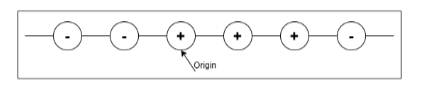
\includegraphics[width=0.5\linewidth]{drawio.png}
    \label{fig:enter-label}
\end{figure}


\begin{enumerate}
    \item[(a)] Find a feature map $\phi : \mathbb{R}^1 \to \mathbb{R}^2$ that maps the data in the original 1-D input space $x$ to a 2-D feature space $\phi(x) = (y_1, y_2)$ so that the data becomes linearly separable. Plot the dataset after mapping in the 2-D space. \hfill (8 points)
   
    we are given the following dataset in 1-D space:
    \[
    \text{Positive data points: } \{0, 1, 2\}, \quad \text{Negative data points: } \{-2, -1, 3\}.
    \]
    to transform the data into a linearly separable form, we can use the kernel function: polynomial kernel of degree 2:
    \[
    \phi(x) = (y_1, y_2) = (x, x^2).
    \]
    to transform the Positive data points:
    \\ the first positive data point is 0:
    \[
    \phi(0) = (0, 0^2) = \textbf{(0, 0)}
    \]
    the second positive data point is 1:
    \[
    \phi(1) = (1, 1^2) = \textbf{(1, 1)}
    \]
    the third positive data point is 2:
    \[
    \phi(2) = (2, 2^2) = \textbf{(2, 4)}
    \]
    to transform the Negative data points:
    \\ the first negative data point is -2:
    \[
    \phi(-2) = (-2, (-2)^2) = \textbf{(-2, 4)}
    \]
    the second negative data point is -1:
    \[
    \phi(-1) = (-1, (-1)^2) = \textbf{(-1, 1)}
    \]
    the third negative data point is 3:
    \[
    \phi(3) = (3, 3^2) = \textbf{(3, 9)}
    \]
    the transformed dataset in 2-D space is:
    \[
    \text{Positive data points: } \{(0, 0), (1, 1), (2, 4)\}, \quad \text{Negative data points: } \{(-2, 4), (-1, 1), (3, 9)\}.
    \]
    the plot of the dataset after mapping in the 2-D space is shown below:
   \(\textbf{Note: }\)  the figure might have floated to a different page.
    \begin{figure}[h!]
        \centering
        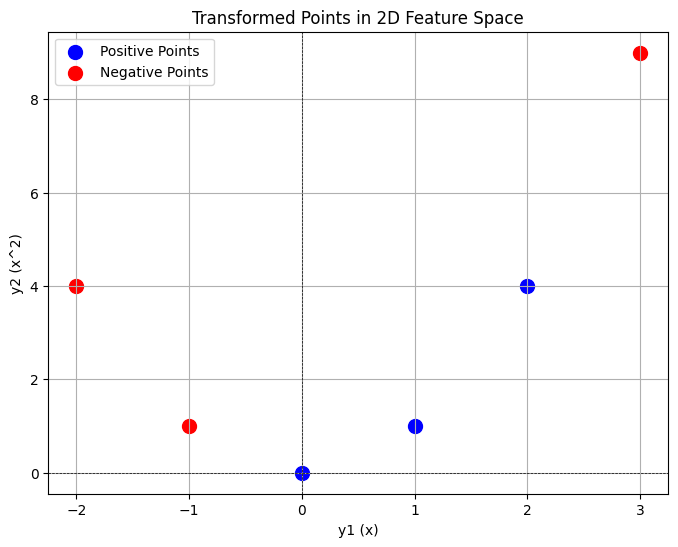
\includegraphics[width=0.5\linewidth]{2D_space.png}
    \label{fig:2D space}
    \end{figure}
    


    \item[(b)] Write down the equation for the separating hyperplane, 
    \(
    w_0 + w_1y_1 + w_2y_2 = 0
    \),
    given by a hard-margin linear SVM in the 2-D feature space. Draw this hyperplane on your plot and mark the corresponding support vector(s). \hfill (12 points)
    \\ the equation for the separating hyperplane is given by:
    \[
    w_0 + w_1y_1 + w_2y_2 = 0
    \]
    where \(w_0\) = bias, \(w_1\) = weight for feature \(y_1\), and \(w_2\) = weight for feature \(y_2\). This is what we are trying to find out so that we can find a hyperplane that separates the positive and negative data points in the 2-D feature space.
    \\ the equation for the separating hyperplane in the 2-D feature space is:
    \[
    w_0 + w_1y_1 + w_2y_2 = 0
    \]
    The optimization problem we are trying to solve is:
    \[
    \min_{w, b} \frac{1}{2} ||w||^2
    \]
    this is subject to the constraints:
    \[
    y_i(w^\top \phi(x_i) + b) \geq 1, \quad \forall i
    \]
    where:
    \(w\) is the weight vector \([w_1, w_2]\), \(b\) = bias, and \(\phi(x_i) = [y_1, y_2]\). are the transformed data points. Also, \(y_i\) is the class label for the data point \(x_i\). For the positive data points, \(y_i = 1\), and for the negative data points, \(y_i = -1\).
    \\ The data points in the 2-D feature space are:
    \[
    \text{Positive data points: } \{(0, 0), (1, 1), (2, 4)\}, \quad \text{Negative data points: } \{(-2, 4), (-1, 1), (3, 9)\}.
    \]
    The labels as mentioned above are:
    \[
    \text{Positive data points: } \{1, 1, 1\}, \quad \text{Negative data points: } \{-1, -1, -1\}.
    \]
    now, the lagrangian function for the optimization problem is:
    \\ \(\textbf{note:}\) why lagrangian? because we are solving a constrained optimization problem. so we need to incoporate the constraints into the objective function.
    \[
    L(w, b, \alpha) = \frac{1}{2} ||w||^2 - \sum^N_{i=1} \alpha_i \big[y_i(w^\top \phi(x_i) + b) - 1\big]
    \]
    where \(\alpha_i\) are the lagrange multipliers.
    \\ the optimal weight vector \(w\) and bias \(b\) are obtained by minimizing the lagrangian function with respect to \(w\) and \(b\), and setting the derivatives to zero:
    \[
    \frac{\partial L}{\partial w} = w - \sum^N_{i=1} \alpha_i y_i \phi(x_i) = 0
    \]
    \[
    \frac{\partial L}{\partial b} = -\sum^N_{i=1} \alpha_i y_i = 0
    \]
    substituting the values of \(w\) and \(b\) back into the lagrangian function, we get the dual optimization problem:
    \[
    \max_{\alpha} \sum^N_{i=1} \alpha_i - \frac{1}{2} \sum^N_{i=1} \sum^N_{j=1} \alpha_i \alpha_j y_i y_j \phi(x_i)^\top \phi(x_j)
    \]
    subject to the constraints:
    \[
    \alpha_i \geq 0, \quad \forall i
    \]
    \[
    \sum^N_{i=1} \alpha_i y_i = 0
    \]
    the optimal weight vector \(w\) and bias \(b\) are obtained by:
    \[
    w = \sum^N_{i=1} \alpha_i y_i \phi(x_i)
    \]
    \[
    b = y_i - w^\top \phi(x_i)
    \]
    computing the kernel matrix:
    \[
    K = \begin{bmatrix}
    \phi(x_1)^\top \phi(x_1) & \phi(x_1)^\top \phi(x_2) & \phi(x_1)^\top \phi(x_3) & \phi(x_1)^\top \phi(x_4) & \phi(x_1)^\top \phi(x_5) & \phi(x_1)^\top \phi(x_6) \\
    \phi(x_2)^\top \phi(x_1) & \phi(x_2)^\top \phi(x_2) & \phi(x_2)^\top \phi(x_3) & \phi(x_2)^\top \phi(x_4) & \phi(x_2)^\top \phi(x_5) & \phi(x_2)^\top \phi(x_6) \\
    \phi(x_3)^\top \phi(x_1) & \phi(x_3)^\top \phi(x_2) & \phi(x_3)^\top \phi(x_3) & \phi(x_3)^\top \phi(x_4) & \phi(x_3)^\top \phi(x_5) & \phi(x_3)^\top \phi(x_6) \\
    \phi(x_4)^\top \phi(x_1) & \phi(x_4)^\top \phi(x_2) & \phi(x_4)^\top \phi(x_3) & \phi(x_4)^\top \phi(x_4) & \phi(x_4)^\top \phi(x_5) & \phi(x_4)^\top \phi(x_6) \\
    \phi(x_5)^\top \phi(x_1) & \phi(x_5)^\top \phi(x_2) & \phi(x_5)^\top \phi(x_3) & \phi(x_5)^\top \phi(x_4) & \phi(x_5)^\top \phi(x_5) & \phi(x_5)^\top \phi(x_6) \\
    \phi(x_6)^\top \phi(x_1) & \phi(x_6)^\top \phi(x_2) & \phi(x_6)^\top \phi(x_3) & \phi(x_6)^\top \phi(x_4) & \phi(x_6)^\top \phi(x_5) & \phi(x_6)^\top \phi(x_6) \\
    \end{bmatrix}
    \]
    where \(\phi(x_1) = (0, 0)\), \(\phi(x_2) = (1, 1)\), \(\phi(x_3) = (2, 4)\), \(\phi(x_4) = (-2, 4)\), \(\phi(x_5) = (-1, 1)\), and \(\phi(x_6) = (3, 9)\).
    \[
    K = \begin{bmatrix}
        (0, 0)\dot (0,0) & (0, 0)\dot (1, 1) & (0, 0)\dot (2, 4) & (0, 0)\dot (-2, 4) & (0, 0)\dot (-1, 1) & (0, 0)\dot (3, 9) \\
        (1, 1)\dot (0,0) & (1, 1)\dot (1, 1) & (1, 1)\dot (2, 4) & (1, 1)\dot (-2, 4) & (1, 1)\dot (-1, 1) & (1, 1)\dot (3, 9) \\
        (2, 4)\dot (0,0) & (2, 4)\dot (1, 1) & (2, 4)\dot (2, 4) & (2, 4)\dot (-2, 4) & (2, 4)\dot (-1, 1) & (2, 4)\dot (3, 9) \\
        (-2, 4)\dot (0,0) & (-2, 4)\dot (1, 1) & (-2, 4)\dot (2, 4) & (-2, 4)\dot (-2, 4) & (-2, 4)\dot (-1, 1) & (-2, 4)\dot (3, 9) \\
        (-1, 1)\dot (0,0) & (-1, 1)\dot (1, 1) & (-1, 1)\dot (2, 4) & (-1, 1)\dot (-2, 4) & (-1, 1)\dot (-1, 1) & (-1, 1)\dot (3, 9) \\
        (3, 9)\dot (0,0) & (3, 9)\dot (1, 1) & (3, 9)\dot (2, 4) & (3, 9)\dot (-2, 4) & (3, 9)\dot (-1, 1) & (3, 9)\dot (3, 9) \\
    \end{bmatrix}
    \]
    \[
    K = \begin{bmatrix}
        0 & 0 & 0 & 0 & 0 & 0 \\
        0 & 2 & 6 & 2 & 0 & 12 \\
        0 & 6 & 20 & 12 & 2 & 42 \\
        0 & 2 & 12 & 20 & 6 & 30 \\
        0 & 0 & 2 & 6 & 2 & 6 \\
        0 & 12 & 42 & 30 & 6 & 90 \\
    \end{bmatrix}
    \]
    now we can solve the dual optimization problem to find the optimal lagrange multipliers \(\alpha_i\).
    \[
    \max_{\alpha} \sum^N_{i=1} \alpha_i - \frac{1}{2} \sum^N_{i=1} \sum^N_{j=1} \alpha_i \alpha_j y_i y_jK_{ij}
    \]
    K is the kernel matrix we computed above.
    \\ labels y are: \(\{1, 1, 1, -1, -1, -1\}\)
    \\ the optimal lagrange multipliers \(\alpha_i\) are:
    \[
    \alpha = [0.456394294 , 0.0.0000000285567450, 0.654716870, 0.0000000100924677, 0.839308304, 0.271802878]
    \]
    the optimal weight vector \(w\) is:
    \[
    w = \sum^N_{i=1} \alpha_i y_i \phi(x_i)
    \]
    \begin{align*}
    w &= 0.456394294 (1)\times [0, 0] \\
    &+ 0.0000000285567450 (1)\times [1, 1] \\
    &+ 0.654716870 (1)\times [2, 4] \\
    &+ 0.0000000100924677 (-1)\times [-2, 4] \\
    &+ 0.839308304 (-1)\times [-1, 1] \\
    &+ 0.271802878 (-1)\times [3, 9] \\
    \end{align*}

\[
 = [0,0] + [0.0000000285567450, 0.0000000285567450] + [1.309433740, 2.618867480] + [0.0000000201849354, -0.0000000403698708]
\]
\[
 + [0.839308304, -0.839308304] + [-0.271802878, -2.446225902] = [1.33333346, -0.66666674]
\]

The support vectors are the data points with non-zero Lagrange multipliers. Usually, \(\alpha > 10^{-5}\). The support vectors are:
\[
(0,0) = [0.456394294], \quad (2,4) = [0.839308304], \quad (-1,1) = [0.654716870], \quad (3,9) = [0.271802878]
\]

to choose the bias \(b\), we can use the support vectors:
\[
b = y_i - w^\top \phi(x_i)
\]
\[
b = 1 - [1.382914024, -1.358013882] \cdot [0, 0] = 1 - 0 = 1
\]
so the equation for the separating hyperplane is:
\[
1 + 1.33333346y_1 - 0.66666674y_2 = 0
\]
\[
y_2 = \frac{1.33333346y_1 + 1}{0.66666674} = 2y_1 + 1.5
\]
\[
\mathbf{y_2 = 2y_1 + 1.5}
\]

the plot of the dataset after mapping in the 2-D space with the separating hyperplane is shown below:
    \begin{figure}[h!]
        \centering
        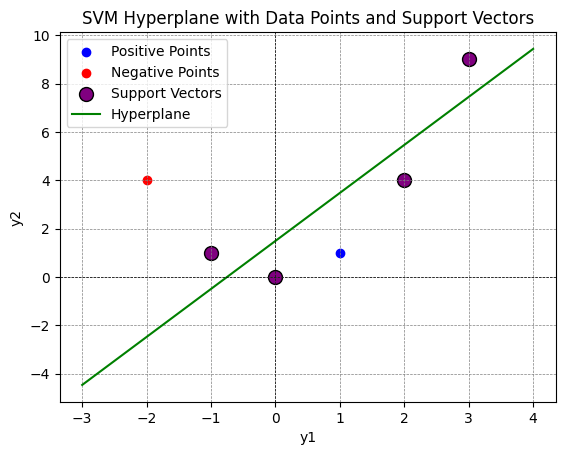
\includegraphics[width=0.5\linewidth]{HYPERLANE.png}
    \label{fig:separating hyperplane}
    \end{figure}
    the support vectors are the data points that lie closest to the separating hyperplane. the support vectors are:
\end{enumerate}

\end{document}